\chapter{实验}
本章主要介绍如何对本文中所提出的补丁兼容性分析方法进行实验,并且给出了实验结果和分析。
\section{实验设计}
\subsection{实验平台}
下面就本文中所采用的实验平台,对其配置说明如下:
\begin{itemize}
	\item 操作系统:Mac OS X 10.9
	\item CPU:2.4 GHz Intel Core i5
	\item 内存:8 GB 1600 MHz DDR3
	\item 硬盘:251 GB APPLE SSD SM0256F Media
\end{itemize}
\subsection{实验数据}

本文中主要采用Eclipse JDT Core项目作为实验对象。JDT Core是Eclipse工具的Java基础组件,它主要提供了如下功能:
\begin{itemize}
	\item Java编译器。
	\item Java文档模型。
	\item Java模型。
	\item 编程帮助。
	\item 搜索。
	\item 源代码排版。
\end{itemize}

该项目的相关信息可以参见表\ref {jdt_core}。

\begin{table}
	\caption{Eclipse JDT Core}
	\label{jdt_core}
	\centering
	\begin{tabular}{llc}
		\toprule[1.5pt]
		{\heiti 信息} & {\heiti 描述} \\\midrule[1pt]
		语言 & Java \\
		文件数 & 约1100个\\
		代码量 & 约3W行\\
		\bottomrule[1.5pt]
	\end{tabular}
\end{table}

Groovy-Eclipse是一个Eclipse的插件集合,用于为Groovy项目提供Eclipse的工具支持。Groovy是一门类似于Java的面向对象编程语言,Groovy代码可以被编译器转化为Java字节码,从而在JVM上运行。由于这一特性,使得Groovy可以调用其他Java语言编写的库,从而大大丰富了其可用性。

Groovy-Eclipse中提供了一个补丁后的JDT Core版本,该补丁主要用于增强JDT Core的功能,使其能够无缝编译Groovy代码。因而我们选择了该补丁作为实验数据中逻辑版本$v_2$的来源。

JDT Core项目截止目前已推出发行版4.4.2,我们从中选择了若干个发行版作为实验数据中逻辑版本$v_1$和$v_3$的来源。逻辑版本的具体说明可以参考表\ref {exp_version},具体的实验数据选择可以参考表\ref {exp_data},其中由于逻辑版本$v_4$由版本合并而来,因此在表\ref {exp_data}中不予列出。

从表\ref {exp_data}中可见,我们一共选择了8个发行版本作为逻辑版本$v_3$的来源。也就是说,我们将以固定的逻辑版本$v_1$和$v_2$为基准,并选择不断变化的逻辑版本$v_3$来进行实验。

这样做的好处是我们可以更加清晰的了解本文中所提出的补丁兼容性分析方法的实用性,包括:
\begin{itemize}
	\item 可针对工业界实际项目进行分析
	\item 切实贴合工业界的实际需求
	\item 对同一软件系统的多个不同版本具有普遍适用性
\end{itemize}

\begin{table}
	\caption{实验数据}
	\label{exp_data}
	\centering
	\begin{tabular}{llc}
		\toprule[1.5pt]
		{\heiti 代码} & {\heiti 发行版本} & {\heiti 逻辑版本} \\\midrule[1pt]
		Eclipse JDT Core & 4.3.2 & $v_1$ \\
		Groovy-Eclipse JDT Core & 4.3.2 & $v_2$\\
		Eclipse JDT Core & 4.4 & $v_3$\\
		Eclipse JDT Core & 4.4.1 & $v_3$\\
		Eclipse JDT Core & 4.4.2 & $v_3$\\
		Eclipse JDT Core & 4.3 & $v_3$\\
		Eclipse JDT Core & 4.3.1 & $v_3$\\
		Eclipse JDT Core & 4.2 & $v_3$\\
		Eclipse JDT Core & 4.2.1 & $v_3$\\
		Eclipse JDT Core & 4.2.2 & $v_3$\\
		\bottomrule[1.5pt]
	\end{tabular}
\end{table}

\begin{table}
	\caption{逻辑版本对照表}
	\label{exp_version}
	\centering
	\begin{tabular}{llc}
		\toprule[1.5pt]
		{\heiti 逻辑版本} & {\heiti 描述} \\\midrule[1pt]
		$v_1$ & 旧版本 \\
		$v_2$ & 应用补丁$p_1$后旧版本\\
		$v_3$ & 新版本\\
		$v_4$ & 版本$v_2$和版本$v_3$合并后版本,相当于应用补丁$p_1$后新版本\\
		\bottomrule[1.5pt]
	\end{tabular}
\end{table}


\section{补丁版本迁移}

所有版本的提交和合并过程可以参考图\ref {exp_git_merge}。

\begin{figure}[H]
	\centering
	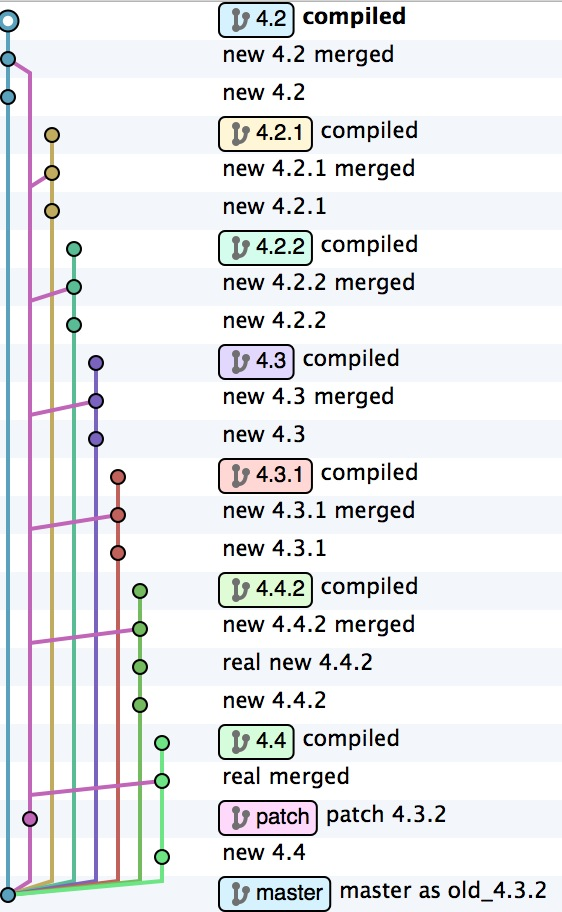
\includegraphics{chap07_git_merge}
	\caption {git版本合并}
	\label {exp_git_merge}	
\end{figure}


在实际执行过程中,需要解决的版本合并冲突可能非常多,由于git在引导第三方工具进行冲突解决时采用的是交互式的策略,因而冲突解决需要花费较长时间和较多人力资源。为此本文采用了Apple Script撰写的脚本来辅助完成这个过程,尽可能的将其自动化。

由于大部分情况下Beyond Compare提供的解决方案都是可行的,因而我们只需要采纳该解决方案即可,如果该工具无法直接提供完全正确的解决方案,则再进行人工解决即可。因而该脚本主要用于自动化实现与图形化GUI工具的交互过程,如下所述。

\begin{lstlisting} [style=BashInputStyle]
tell application "System Events"
	repeat 300 times
		delay 1
		set theName to name of the first process
			whose frontmost is true	
		if theName is "BCompare" then		
			delay 1	
			keystroke "s" using {command down}	
			delay 1	
			if theName is "BCompare" then
				keystroke "w" using {command down}
			end if		
			delay 1		
		else
			delay 1
		end if
	end repeat
end tell


\end{lstlisting}

\section{语义影响范围分析}
\subsection{程序间差异性分析}
\subsection{变更影响分析}
\section{兼容性分析}
\section{结果分析}